\documentclass[final]{beamer}
\usepackage[orientation=portrait,size=a4,scale=1.0]{beamerposter}
\usetheme{gemini}
\usepackage{lipsum}
\usecolortheme{nott}
\usepackage{graphicx}
\usepackage[spanish]{babel}
\usepackage{newtxtext,fourier} 
\usepackage{tikz}
\usepackage{pgfplots}
\pgfplotsset{compat=1.14}
\usepackage{amsmath, amsfonts, amsthm, amssymb}
\newcommand\T{\ensuremath{\mathbb{T}}}
\newcommand\N{\ensuremath{\mathbb{N}}}
\newcommand\R{\ensuremath{\mathbb{R}}}
\newcommand\Z{\ensuremath{\mathbb{Z}}}
\newcommand\Q{\ensuremath{\mathbb{Q}}}
\newcommand\C{\ensuremath{\mathbb{C}}}
\newcommand\Hs{\ensuremath{\mathbb{H}}}
\newlength{\sepwidth}
\newlength{\colwidth}
\setlength{\sepwidth}{0.025\paperwidth}
\setlength{\colwidth}{0.45\paperwidth}
\newcommand{\separatorcolumn}{\begin{column}{\sepwidth}\end{column}}
\newtheorem{teor}{Teorema}
\newcommand{\defi}[1]{\textbf{\emph{#1}}} 
\title{\Huge Espacios de TeichMuller y Moduli}

\author{\Large Sergio Alejandro Bello Torres\\Edgar Santiago Ochoa Quiroga\\Departamento de Matemáticas, Universidad Nacional de Colombia}
\logoleft{
  \begin{tabular}{@{}c@{}}
    \hspace{1.2cm}
\includegraphics[scale=0.05]{logo.jpg} \\
  \end{tabular}
}
\begin{document}
\Large
\begin{frame}[t,fragile]
\begin{columns}[t]
\separatorcolumn

\begin{column}{\colwidth}

\begin{block}{Introducción}
Uno de los problemas principales en el estudio de las superficies de Riemann es su clasificación, en particular hemos visto que una misma superficie puede tener dos estructuras complejas completamente diferentes, por lo que nos interesamos en caracterizar todas estas estructuras. A partir de este problema surgen los espacios de Moduli y Teichmüller, que por su estructura ayudan a clasificar todas las posibles estructuras complejas de una superficie dada. Nuestro propósito es hacer una breve introducción a éstos espacios, incluyendo algunas construcciones elementales.
\end{block}

\begin{exampleblock}{Teorema de Uniformizacion}
Sea $X$ una superficie de Riemann simplemente conexa, entonces $X$ es biholomorfa a exactamente una de las siguientes superficies
        \begin{itemize}
            \item La esfera de Riemann $\C_{\infty}.$
            \item El plano Complejo $\C.$
            \item El semiplano superior $\Hs^2.$
        \end{itemize}
\end{exampleblock}
    
\begin{block}{Cocientes de superficies}
    Como consecuencia del teorema de uniformización, podemos realizar cada superficie de Riemann como un cociente de $\C,\C_\infty$ o $\Hs^2$, más específicamente, tenemos los siguientes resultados:\\
    \vspace{0.2cm}
    \defi{Proposición: }Sea $X$ una superficie de Riemann. El cubrimiento universal de $X$ es biholomorfo a $\C_\infty$ si y solo si $X$ es biholomorfo a $\C_\infty$.\\
    \vspace{0.2cm}
    \defi{Proposición: }Sea $X$ una superficie de Riemann. El cubrimiento universal de $X$ es biholomorfo a $\C$ si y solo si $X$ es biholomorfo a $\C,\C-\{0\}$ o $\C/L$.\\ 
    \vspace{0.2cm}
    De ésto podemos observar que la mayor variedad se encuentra en los cocientes de $\Hs^2$. 
\end{block}    
\begin{alertblock}{Superficies hiperbólicas}
Los cocientes de $\Hs^2$ son lo que denominaremos como superficies hiperbólicas. Se tiene que $\Hs^2$ viene equipado con una métrica dada por
$$ds^2=\dfrac{dx^2+dy^2}{y^2},$$
además, el grupo de automorfismos $\text{PSL}(2,\R)$ de $\Hs^2$, es justamente el grupo de isometrías que preservan la orientación de esta métrica.\\
\vspace{0.3cm}
\defi{Observación:} Todos los cocientes de $\Hs^2$ que dan lugar a una superficie de Riemann heredan una métrica completa de curvatura constante $-1$, es decir una métrica hiperbólica. Más aún, toda métrica de la que se puede dotar una superficie da lugar a una superficie de Riemann.
  \end{alertblock}
\begin{block}{Espacio de Teichmüller del Toro}
    Sabemos que todo toro complejo es isomorfo a un toro determinado por $\{1,\tau\}$ con $\tau \in \Hs^2$, lo cual nos indica que cualquier estructura compleja del toro viene determinada por un punto del plano hiperbólico. Sin embargo, pueden existir $\tau,\tau^{\prime} \in \Hs^2$ con $\tau = \tau^{\prime}$ que resulten en dos estructuras biholomorfas.\\ 
    \vspace{0.2cm}
    \defi{Proposición: } Sean $\C/L$ y $\C/L'$ dos toros determinados por $\tau$ y $\tau'$ respectivamente, entonces son biholomorfos si y solo si
        \[
            \tau' = \frac{a\tau + b}{c\tau + d}
        \]
        Con $a,b,c,d \in \Z$ y $ad-bc=1$.\\ 
    Ésto quiere decir que las estructuras de superficie de Riemann del toro están determinadas por la acción de $\text{SL}(2,\Z)$ sobre $\Hs^2$
\end{block}

\end{column}

\separatorcolumn

\begin{column}{\colwidth}
\begin{block}{Espacio de Moduli del toro}
Sea $\mathcal{M}_1 = \Hs^2/\text{SL}(2,\Z) = \Hs^2/\text{PSL}(2,\Z)$, podemos comprender la topología de este cociente a partir de su dominio fundamental, consideremos el conjunto:
    $$\mathcal{F}=\left\{z\in\Hs^2:|z|\geq 1\text{ y } |Re(z)|\leq \frac{1}{2}\right\}.$$
    \begin{figure}
            \centering
            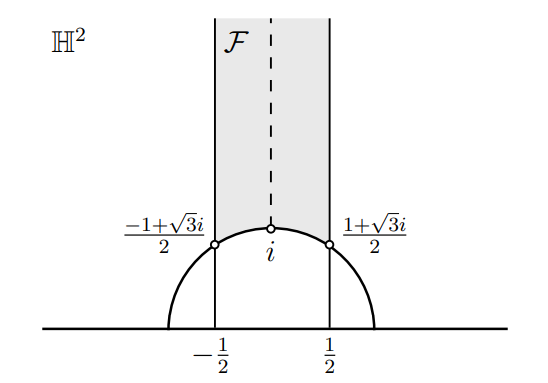
\includegraphics[width=0.7\linewidth]{Imagenes/FunDom.png}
        \end{figure} 
Sea $\tau \in \mathcal{F}$, tenemos lo siguiente:
\begin{itemize}
        \item Si $\tau\in \text{Int}(\mathcal{F})$ entonces $O(\tau)\cap\mathcal{F}=\{\tau\}.$ 
        \item Si $\text{Re}(\tau)=\pm\dfrac{1}{2}$ entonces $O(\tau)\cap\mathcal{F}=\{\tau,\tau\mp1\}.$
        \item Si $|\tau|=1$ entonces $O(\tau)\cap \mathcal{F}=\left\{\tau,-\dfrac{1}{\tau}\right\}.$
    \end{itemize}
Entonces $\mathcal{M}_1$ es el espacio que resulta de identificar los bordes de $\mathcal{F}$, así:
    \begin{figure}
            \centering
            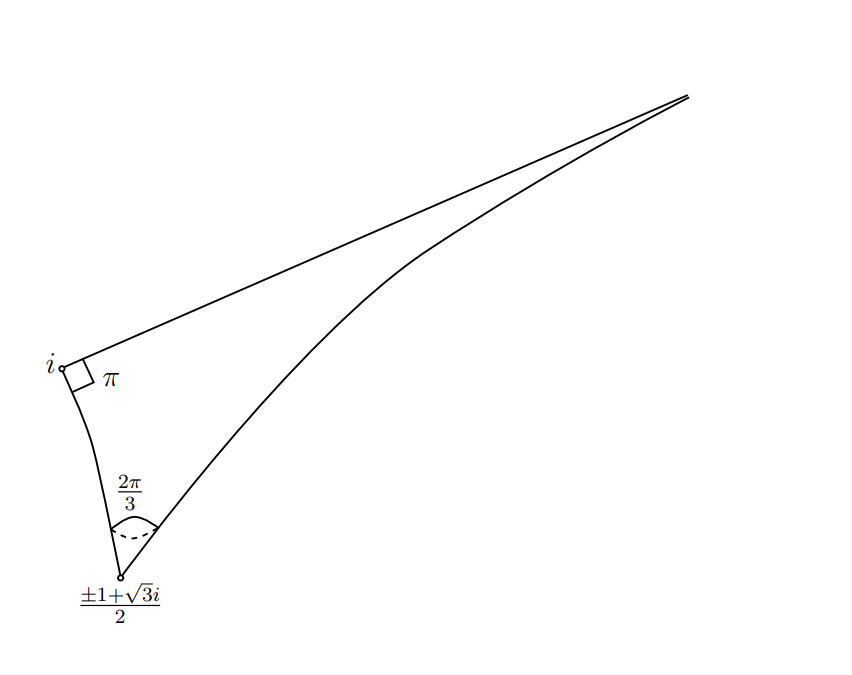
\includegraphics[width=0.7\linewidth]{Imagenes/Empanada.png}
        \end{figure} 

    $\mathcal{M}_1$ se denomina el espacio de móduli del toro y $\mathcal{T}_1 = \Hs^2 $ es el espacio de Teichmüller
\end{block}
\begin{alertblock}{Marking}
    \defi{Definición: }Sea $X$ una superficie de Riemann cerrada género g,  decimos que $\Sigma_g = \{[A_1],[A_2],\ldots,[A_g],[B_1],[B_2],\ldots, [B_g]\}$ es un \textbf{sistema canónico de generadores} para $\pi_1(X,p_0)$ si\\
    $$\prod_{i=1}^g [A_i,B_i] = e$$\\
    \begin{itemize}
        \item Un \textit{marking} en $X$ es un sistema canónico de generadores $\Sigma_p \subset \pi_1(X,p)$
        \item Dos markings $\Sigma_p$ y $\Sigma_{p'}^\prime$ se dicen  \textbf{equivalentes} si existe una curva contínua $\alpha$ entre $p$ y $p'$, tal que el isomorfismo inducido $T_\alpha: \pi_1(X,p) \rightarrow \pi_1(X,p')$ satisface\\
        $$
        T_\alpha(\Sigma_p) = \Sigma_{p^\prime}'.
        $$\\
    \end{itemize}
    Al par $(X,\Sigma_p)$ lo llamamos \textbf{superficie de Riemann marcada}. 
\end{alertblock}
\end{column}

\separatorcolumn

\end{columns}
\end{frame}

\newpage
\thispagestyle{empty}
\vspace*{-1.5cm}

\begin{frame}[t,fragile]
\begin{columns}[t]
\separatorcolumn
\begin{column}{\colwidth}

\begin{block}{Marking por difeomorfismos}
\defi{Definición: }Sean $R$ y $R^\prime$ superficies de Riemann, definamos
            \begin{align*}
                 f:X\to R\,\text{  y  }\,f^\prime:X\to R^\prime,
             \end{align*} 
             como difeomorfismos que preservan la orientación. Decimos que las parejas $(R,f)$ y $(R^\prime,f^\prime)$ son equivalentes si existe un biholomorfismo $h:R\to R^\prime$ tal que
             $$(f^\prime)^{-1}\circ h\circ f:X\to X,$$
             es homotopico a la identidad.\\ 
        \defi{Observación: } Si escogemos un conjunto de generadores $\Sigma$ para el grupo fundamental $\pi_1(X,p)$, entonces cada pareja $(R,f)$ define un punto
        $$(R,f_{*}(\Sigma))\in \mathcal{T}.$$
        Donde $\mathcal{T}$ es el espacio de Teichmüller de $X.$
        Ésta nos brinda una nueva descripción del espacio de Teichmïller de una superficie $X.$
        $$\mathcal{T}(X)=\left\{(R, f): \begin{array}{c}R \text{ es una superficie de Riemann }, f: X \rightarrow R \\ \text{ un difeomorfismo que preserva la orientación }\end{array}\right\} / \sim.$$
        Con esta nueva descripción será mucho mas sencillo describir el espacio de Moduli, con lo que llamaremos \textit{Mapping class group.}
\end{block}

\begin{alertblock}{Mapping class group} 
Sea $X$ una superficie de Riemann cerrada. Definimos\\
       $$Diff^+(X)=\left\{f:X\to X| \begin{array}{c}f \text{ es un difeomorfismo que}\\ \text{preserva la orientación }\end{array}\right\},$$\\
        y
        $$Diff^+_0(X)=\left\{f\in Diff^+(X):f\text{ es homotópico a la identidad}\right\}.$$\\
        Podemos notar que $Diff^+(X)$ es un grupo y que $Diff^+_0(X)$ es un subgrupo normal de $Diff^+(X).$ Con lo cual\\
        \vspace{0.2cm} 
        \defi{Definición: }El \textbf{Mapping class group} de una superficie de riemann cerrada $X$ es
            $$\text{MCG}(X):=Diff^+(X)/Diff^+_0(X).$$\\ 
        \vspace{0.2cm}
        El \textit{Mapping class group} actua sobre el espacio de Teichmüller de la siguiente manera:
        $$[g]\cdot[(R,f)]=[(R,f\circ g^{-1})].$$
        El cociente de el espacio de Teichmüller por esta acción es lo que llamaremos espacio de Moduli, es decir
            El \textbf{espacio de Moduli} de una superficie de Riemann cerrada $X$ es
            $$\mathcal{M}(X)=\mathcal{T}(X)/\text{MCG}(X).$$
    
\end{alertblock}

\begin{block}{Aplicaciones conformes y cuasiconformes}
    \defi{Definición: } Sea $f: D \rightarrow D^{\prime}$ un difeomorfismo que preserva la orientación de un dominio $D$ del plano complejo a otro $D'$. Definimos la $\textbf{dilatación}$ de $f$ en el punto $z$ como 
    $$D_f=\frac{|f_z|+|f_{\overline{z}}|}{|f_z|-|f_{\overline{z}}|}\geq 1.$$\\ 

    $f$ se dice cuasiconforme si $D_f$ es acotada, particularmente tenemos que $f$ es conforme si $D_f=1$. 
\end{block}


\end{column}

\separatorcolumn

\begin{column}{\colwidth}
\phantom{xd}\\ \vspace{0.85cm}
Nos resulta más conveniente considerar 
     $$d_f=\frac{|f_{\overline{z}}|}{|f_z|}<1,$$
    que se relaciona con $D_f$ tal que
    $$D_f=\frac{1+d_f}{1-d_f}.$$
\defi{Definición: } La \text{dilatación compleja} esta dada por
        $$\mu_f=\frac{f_{\overline{z}}}{f_z}.$$
        LLamamos a $\mu_f$ el \textit{coeficiente de Beltrami de }$f.$
\begin{exampleblock}{Espacios de coeficientes de Beltrami}
\defi{Proposición: }Dadas superficies de Riemann $R,S,T,$ y difeomorfismos que preservan la orientación $f:R\to S$ y $g:S\to T$, se tiene la siguiente relación
        $$\mu_g\circ f=\frac{f_z}{\overline{f_z}}\frac{\mu_{g\circ f}-\mu_f}{1-\overline{\mu_f}\cdot\mu_{g\circ f}}.$$ 
        Es particular si tenemos difeomorfismos que preservan la orientación $f_1:R\to S_1$ y $f_2:R\to S_2$, la aplicacion $f_2\circ f_1^{-1}$ es biholomorfa si y solo si $\mu_{f_1}=\mu_{f_2}.$\\
    Sea $B(X)_1$ el conjunto de los coeficientes de Beltrami de $X$, si equipamos a este conjunto con la norma $L^\infty$, hemos definido una topología. Consideramos la acción de $Diff^+(X)$ sobre $B(X)_1$, dada por
    $$w^*(\mu_f)=\mu_{f\circ w^{-1}}=\left(\frac{w_z}{\overline{w_z}}\frac{\mu_f-\mu_w}{1-\overline{\mu_w}\mu_f}\right)\circ w^{-1},$$
    \defi{Teorema: }Dados difeomorfismos que preservan la orientación $f:X\to R$ y $g:X\to R^\prime$, existe una aplicacion biholomorfa $h:R\to R^\prime$ si y solo si existe $w\in Diff^+(X)$ tal que $\mu_g=w^*(\mu_f).$ Ademas $g^{-1}\circ h\circ f$ es homotopico a la identidad en $X$ si y solo si $w\in Diff_0^+(X).$\\ 
    \defi{Corolario: }La aplicación que envia $(R,f)$ a $\mu_f\in B(X)_1$ induce las siguientes correspondencias
        \begin{align*}
           \mathcal{T}(X)&\cong B(X)_1/Diff_0^+(X),\\
           \mathcal{M}(X)&\cong B(X)_1/Diff^+(X). 
        \end{align*}
\end{exampleblock}
\begin{alertblock}{Problema de Grötschz}
    Sean $R,R^\prime$ dos rectángulos de lados $a,b$ y $a^\prime,b^\prime$ respectivamente. Queremos ver cual es la aplicación $f$ que enviá $R\to R^\prime$, que sea lo mas conforme posible, con conforme nos referimos a que la norma de la dilatación $D_f$ sea mínima.\\
    \defi{Teorema: }        Sea 
        $$f(z)=\frac{1}{2}\left(\frac{a^\prime}{a}+\frac{b^\prime}{b}\right)z+\frac{1}{2}\left(\frac{a^\prime}{a}-\frac{b^\prime}{b}\right)\overline{z},$$
        entonces $f(z)$ es solución para el problema de Grötschz.\\ 
\end{alertblock}
\begin{block}{Referencias}
        \begin{thebibliography}{9}

\bibitem{ahlfors}
L. V. Ahlfors, \textit{Lectures on Quasiconformal Mappings}, D. Van Nostrand Company, 1966.

\bibitem{petri}
B. Petri, \textit{Introduction to Teichmüller Theory. Lecture Notes}, 2024.

\bibitem{Imayoshi}
Y. Imayoshi, M. Taniguchi, \textit{An Introduction to Teichmüller Spaces}, Springer, 1992.


\end{thebibliography}
\end{block}
\end{column}

\separatorcolumn

\end{columns}
\end{frame}


\end{document}
